\chapter{Fractal Tree}

\noindent Fractal Tree është një fraktal i njohur që përfaqëson vizualisht konceptin e rekursionit në natyrë. Ndërtimi i këtij fraktali fillon me një trung të vetëm, i cili më pas ndahet në dy degë në një kënd të caktuar. Secila prej këtyre degëve ndahet më tej në dy degë më të vogla, duke vazhduar këtë proces në mënyrë rekursive \cite{fractal_geometry}. Iterimet e para të këtij fraktali janë  paraqitur në figurën \ref{fig:tree_grow}. Me rritjen e iterimeve do të fitohet figura \ref{fig:tree_big}.

\begin{figure}[htbp!]
\centering
\subfigure[Iterimi 2]{\includegraphics[width=83px,height=90px]{tree_1}}
\subfigure[Iterimi 4]{\includegraphics[width=83px,height=90px]{tree_2}}
\subfigure[Iterimi 7]{\includegraphics[width=83px,height=90px]{tree_3}}
\subfigure[Iterimi 7]{\includegraphics[width=83px,height=90px]{tree_4}}
\caption{Rritja e pemës fraktale}
\label{fig:tree_grow}
\end{figure}

\section{Konstruktimi i degëve}

Le të jenë pikat \( A(x_1, y_1) \) dhe \( B(x_2, y_2) \). Duhet të gjejmë pikën \( C(c_1, c_2) \) ashtu që \( \overrightarrow{AB} = \lambda \overrightarrow{BC} \), dhe pikat \( C' \) dhe \( C'' \) ashtu që \( \angle CBC' = \alpha = \angle CBC'' \) (figura \ref{fig:fractal_construction}).


\begin{figure}[htpb]
    \centering
    \includegraphics[width=1\linewidth]{tree_5.png}
    \caption{Konstruktimi i degës.}
    \label{fig:fractal_construction}
\end{figure}



\noindent \\ Nga barazimi \( \overrightarrow{AB} = \lambda \overrightarrow{BC} \) marrim

\[
(x_2 - x_1, y_2 - y_1) = \lambda (c_1 - x_2, c_2 - y_2)
\]

\noindent \\ Duke barazuar kordinatat përkatëse të dysheve të renditura në të dy anët e barazimit marrim

\[
x_2 - x_1 = \lambda (c_1 - x_2)
\]
\[
y_2 - y_1 = \lambda (c_2 - y_2)
\]


\noindent \\Duke zgjidhur për \(c_1\), \(c_2\) fitojmë:

\[
c_1 = \frac{x_2 (1 + \lambda) - x_1}{\lambda}
\]

\[
c_2 = \frac{y_2 (1 + \lambda) - y_1}{\lambda}
\]

\noindent \\ Pikën \( C \) e rrotullojmë rreth pikës \( B \) për këndin \( \alpha \) dhe fitojmë pikën \( C'' \) me koordinatat:

\[
c_1'' = (c_1 - x_2) \cos(\alpha) - (c_2 - y_2) \sin(\alpha) + x_2
\]

\[
c_2'' = (c_1 - x_2) \sin(\alpha) + (c_2 - y_2) \cos(\alpha) + y_2
\]


\noindent \\ Ngjashëm, pika \( C' \) fitohet duke rrotulluar pikën \( C \) rreth pikës \( B \) për këndin \(-\alpha\).





\section{Numri i pikave të figurës}

\noindent \\ Le të jetë \( f(n) \) numri i brinjëve të figurës në iterimin \( n \). Pas secilit iterim, numri i brinjëve dyfishohet dhe kemi:

\[ f(n) = 2^0 + 2^1 + 2^2 + \cdots + 2^n = 2^{n+1} - 1. \]

\noindent \\ Secila brinjë ka dy pika dhe numri i pikave do të jetë \( 2 \cdot f(n) \), dhe këtë shprehje e përdorim për të lidhur pikat si segmente në pjesën e vizualizimit. \\

\begin{lstlisting}
void renderTreeFromBuffer() {
    glVertexAttribPointer(0, 2, GL_FLOAT, GL_FALSE, 0, nullptr);
    glEnableVertexAttribArray(0);
    glColor3f(0.0f, 0.0f, 0.0f);
    int numberOfVertices = 2 * (pow(2, iteration + 1) - 1);
    glDrawArrays(GL_LINES, 0, numberOfVertices2(iterations));
    glutSwapBuffers();	
}
\end{lstlisting}

\section{Paralelizimi}
\noindent Paralelizimi ndodh në menyrë hiearkike, ku në secilin iterim do të jenë aktiv një numër i caktuar i thredave. Secili thread aktiv do e marë degën  e \(i\) -të të figurës, dhe do e konstruktoj degën e djathtë ose të majtë varësisht nga indeksi. Dega e re e fituar futet në vargun e të gjitha degëve. Madhësia e këtij vargu do të jetë \( f(n) \).

\noindent \\ Për secilin iterim do të jenë \(2^n \) threada aktiv. Me rritje të iterimeve, numri i thredave aktiv do të  ngritet eksponencialisht: 

\begin{enumerate}
    \item Iterimi 0: Vetëm threadi me id 0 të jetë aktiv. Ky thread inicalizon degën fillestare.
    \item Iterimi 1: Threadat 2 dhe 3 janë aktiv. Threadi 2 konstrukton degën e majtë nga dega fillestare dhe e fut në vargun e degëve në pozitën 2. Threadi 3 do konstrukton degën e djathtë dhe e fut në vargun e degëve në pozitën 3.
    \item Iterimi 2: Threadat 4,5,6,7 janë aktiv. Thredat 3 dhe 4 konstruktojnë dëgën e majtë dhe të djathtë të degës nga pozita 2 e vargut.  Thredat 5,6 konsturktojnë degën e majtë dhe të djathtë, rrespektivisht, të degës nga pozita 3 e vargut. Deget e krijuara futen në vargun e degëve për iterimin e ardhshëm. 
    \item Iterimi \(n\): Threadat \(2^n\) deri në \(2^{n+1}-1\) do të jenë aktiv. Këta threada marin degët përkatëse, dhe varësisht nga indeksi konstruktojnë degë të djathtë ose të majtë.  
\end{enumerate}


\begin{figure}[htbp]
    \centering
    \includegraphics[width=1\linewidth]{tree_6.png}
    \caption{Ekzekutimi paralel i thredave.}
    \label{fig:tree_threads}
\end{figure}


\noindent \\ Paralelizimi dhe shtimi i të dhënave është modeluar në një graf binar (figura \ref{fig:tree_threads}). Çdo nyje në graf përfaqëson një thread që ndërton një degë, ndërsa degët e grafit përfaqësojnë ndarjen degës në iteracionet e ardhshme. Secili thread \(i\)  merr degën nga pozicioni prind \(i/2\) nga vargu i degëve, e konstrukton degën e djathtë ose të majtë, dhe dega e re e konstruktuar futet në pozicionin  \(i\)  të vargut. Secili nivel i grafit përfaqëson threadat të cilët janë duke punuar në paralel. 

\noindent \\ Indeksi më i majtë në nivelin \(n\) të grafit është:
\[ \text{leftMost}(n) = 2^n \]
\noindent Indeksi më i djathtë në nivelin \(n\) të grafit është:
\[ \text{rightMost}(n) = \text{leftMost}(n+1) - 1 = 2^{n+1} - 1 \]
\noindent  Numri i thredave që punojnë në paralel në nivelin \(n\) është:
\[ \text{leftMost}(n+1) - \text{leftMost}(n) = 2^{n+1} - 2^n = 2^n \]

\section{Kerneli}

\noindent Kerneli i mëposhtëm gjeneron fraktalin përmes llogaritjes paralele. Fillimisht threadi me indeks 0 trajton degën inicializuese. Për secilin iterim threads ndërmjet intervalit start\_at dhe end\_at janë aktiv dhe konstruktojnë degët e reja. Threads me indeks numër çift konstruktojnë degët e majta, kurse thredat me numër tek konstruktojnë degët e djathta.  Degët e konstruktuara ruhen në vargun e degëve të cilat do të ndahen në iterimin e ardshëm. Dy kulmet e degës i shtohen vargut points. Sinkronizimi siguron që të gjitha threadat përfundojnë detyrën e tyre para sa te të vazhdojnë në iterimin e ardhshëm. \\

\begin{lstlisting}
__global__ void branchDivide(float* points, Branch branch, Branch* branches, float angle_left, float angle_right, int start_iteration, int max_iterations, int threadShiftIndex) {

    int idx = threadIdx.x + blockIdx.x * blockDim.x;;
    idx += threadShiftIndex;
    
    Branch childBranch,parentBranch;
    float angle;
    auto g = cg::this_grid();
    
    if (idx == 0) {
        points[0] = branch.start.x;
        points[1] = branch.start.y;
        points[2] = branch.end.x;
        points[3] = branch.end.y;
        branches[1] = branch;
    }
    
    for (int iteration = start_iteration; iteration <= max_iterations; iteration++) {
        float start_at = round(pow(2, iteration));
        int end_at = round((pow(2, iteration + 1))) - 1;
    
        if (idx >= start_at && idx <= end_at) {
            int parentNode = idx / 2;
            parentBranch = branches[parentNode];
            int t = idx % 2;
            
            if (t == 0) {
                angle = angle_left;
            }
            else {
                angle = angle_right;
            }
            
            childBranch = makeChildBranch(parentBranch,angle);
            branches[idx] = childBranch;
            //add points to points array;
            int offset = 2 * 2 * (idx - 1);
            points[offset] = childBranch.start.x;
            points[offset + 1] = childBranch.start.y;
            points[offset + 2] = childBranch.end.x;
            points[offset + 3] = childBranch.end.y;
        }
    g.sync();
    }
}
\end{lstlisting}

\section{Krahasimet}

 Tabela \ref{tab:tree_table} krahason kohën e ekzekutimit në mikrosekonda të fraktalit ndërmjet versionit sekuencial dhe të versionit paralel. Implementimi me CUDA është bërë me  anë të grupeve kooperative, me 23040 threada për një thirrje të kernelit. Vizualizimi i këtyre rezultateve është në figurën \ref{fig:tree_graph}.
 
\begin{table}[h]
\centering
\resizebox{0.3\textwidth}{!}{%
\begin{tabular}{|l|l|l|}
\hline
Iterimi & C++ & CUDA \\ \hline
0 & 23 & 27 \\ \hline
1 & 40 & 25 \\ \hline
2 & 47 & 23 \\ \hline
3 & 39 & 28 \\ \hline
4 & 40 & 27 \\ \hline
5 & 58 & 27 \\ \hline
6 & 332 & 29 \\ \hline
7 & 288 & 28 \\ \hline
8 & 105 & 26 \\ \hline
9 & 155 & 26 \\ \hline
10 & 436 & 27 \\ \hline
11 & 541 & 24 \\ \hline
12 & 733 & 29 \\ \hline
13 & 1563 & 29 \\ \hline
14 & 2576 & 43 \\ \hline
15 & 4861 & 47 \\ \hline
16 & 9027 & 89 \\ \hline
17 & 22230 & 148 \\ \hline
18 & 37435 & 253 \\ \hline
19 & 75886 & 382 \\ \hline
20 & 145146 & 745 \\ \hline
21 & 294950 & 1268 \\ \hline
22 & 584644 & 2560 \\ \hline
23 & 1184101 & 5265 \\ \hline
24 & 2347734 & 142678 \\ \hline
25 & 4705941 & 439919 \\ \hline
26 & 9416423 & 789610 \\ \hline
\end{tabular}
}
\caption{Krahasimi i performancës.}
\label{tab:tree_table}
\end{table}

\begin{figure}[h]
\centering
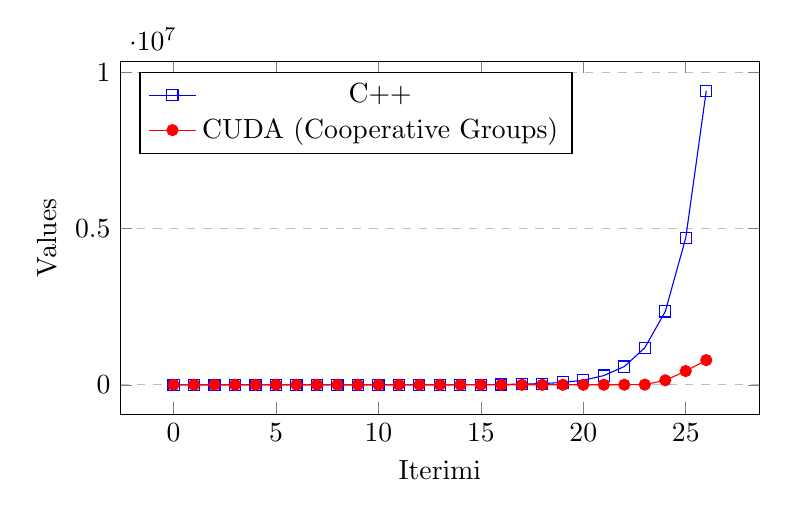
\begin{tikzpicture}
\begin{axis}[
    title={},
    xlabel={Iterimi},
    ylabel={Values},
    legend pos=north west,
    ymajorgrids=true,
    grid style=dashed,
    width=0.8\textwidth,  % Adjust width as needed
    height=0.5\textwidth, % Adjust height as needed
]
\addplot[
    color=blue,
    mark=square,
    ]
    coordinates {
    (0,23)(1,40)(2,47)(3,39)(4,40)(5,58)(6,332)(7,288)(8,105)(9,155)(10,436)(11,541)(12,733)(13,1563)(14,2576)(15,4861)(16,9027)(17,22230)(18,37435)(19,75886)(20,145146)(21,294950)(22,584644)(23,1184101)(24,2347734)(25,4705941)(26,9416423)
    };
\addplot[
    color=red,
    mark=*,
    ]
    coordinates {
    (0,27)(1,25)(2,23)(3,28)(4,27)(5,27)(6,29)(7,28)(8,26)(9,26)(10,27)(11,24)(12,29)(13,29)(14,43)(15,47)(16,89)(17,148)(18,253)(19,382)(20,745)(21,1268)(22,2560)(23,5265)(24,142678)(25,439919)(26,789610)
    };
\legend{C++, CUDA (Cooperative Groups)}
\end{axis}
\end{tikzpicture}
\caption{Grafiku i krahasimit të performancës.}
\label{fig:tree_graph}
\end{figure}



\newpage


% \begin{figure}
%     \centering
%     \includegraphics[width=0.90\linewidth]{tree_7.png}
%     \caption{Enter Caption}
%     \label{fig:enter-label}
% \end{figure}


\begin{figure}[]
    \centering
    \makebox[\textwidth]{\includegraphics[width=1.7\linewidth]{tree_7.png}}
    \caption{Pema fraktale në iterimin 24 e gjeneruar me CUDA.}
    \label{fig:tree_big}
\end{figure}
